\documentclass[tikz,border=2pt]{standalone}
\usepackage{times}
\usepackage{amsmath}
\usepackage{pgfplots}
\pgfplotsset{compat=1.16}
\begin{document}
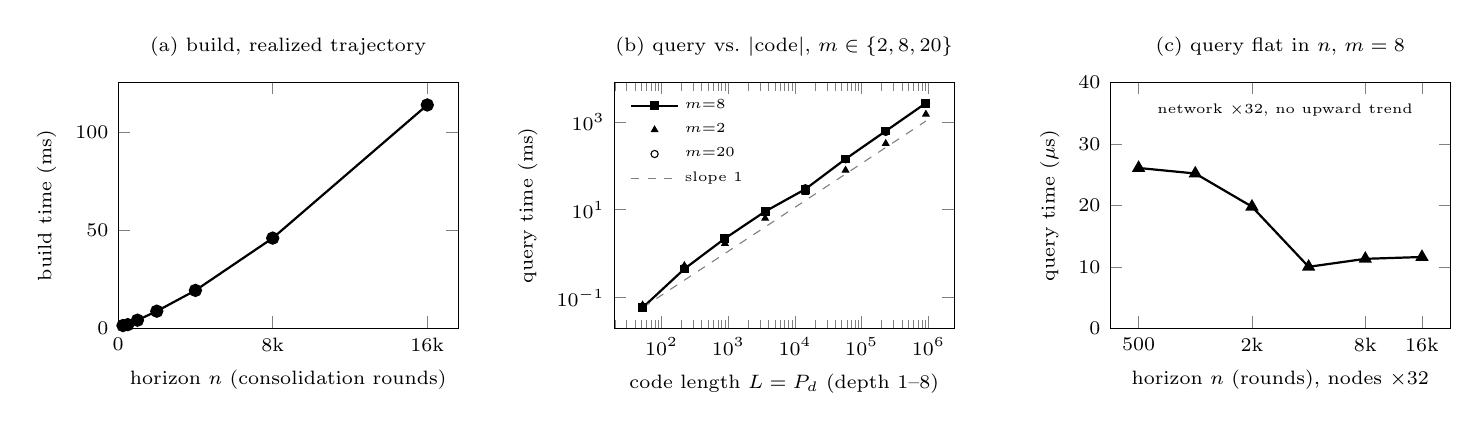
\begin{tikzpicture}
% (a) build time vs n (integer-coded realized trajectory) -- linear
\begin{axis}[
  width=5.9cm, height=4.7cm, font=\scriptsize,
  xlabel={horizon $n$ (consolidation rounds)}, ylabel={build time (ms)},
  ymin=0, xmin=0,
  scaled x ticks=false,
  title={\scriptsize (a) build, realized trajectory},
  xtick={0,8000,16000}, xticklabels={0,8k,16k},
]
\addplot[mark=*, thick] coordinates {(250,1.36)(500,1.82)(1000,4.09)(2000,8.69)(4000,19.31)(8000,46.03)(16000,114.04)};
\end{axis}
% (b) query time vs code length L=P_d (abstract padded codes), scaled by depth -- poly in L
\begin{scope}[xshift=6.3cm]
\begin{axis}[
  width=5.9cm, height=4.7cm, font=\scriptsize,
  xlabel={code length $L=P_d$ (depth 1--8)}, ylabel={query time (ms)},
  xmode=log, ymode=log,
  title={\scriptsize (b) query vs.\ $|\text{code}|$, $m\in\{2,8,20\}$},
  legend style={font=\tiny, at={(0.02,0.98)}, anchor=north west, draw=none, fill=none},
  legend cell align=left,
]
\addplot[mark=square*, mark size=1.2pt, thick] coordinates {(52,0.059)(220,0.450)(892,2.222)(3580,9.151)(14332,29.46)(57340,142.98)(229372,616.98)(917500,2665.07)};
\addlegendentry{$m{=}8$}
\addplot[mark=triangle*, mark size=1.3pt, only marks] coordinates {(52,0.068)(220,0.535)(892,1.711)(3580,6.394)(14332,24.67)(57340,79.13)(229372,320.58)(917500,1487.01)};
\addlegendentry{$m{=}2$}
\addplot[mark=o, mark size=1.3pt, only marks] coordinates {(52,0.061)(220,0.477)(892,2.275)(3580,9.279)(14332,30.82)(57340,140.81)(229372,590.21)(917500,2638.43)};
\addlegendentry{$m{=}20$}
\addplot[domain=52:917500, dashed, gray, samples=2] {0.059/52*x};
\addlegendentry{slope $1$}
\end{axis}
\end{scope}
% (c) flat query vs n (integer-coded) -- horizon-independent
\begin{scope}[xshift=12.6cm]
\begin{axis}[
  width=5.9cm, height=4.7cm, font=\scriptsize,
  xlabel={horizon $n$ (rounds), nodes $\times32$}, ylabel={query time ($\mu$s)},
  xmode=log, log basis x=2, ymin=0, ymax=40,
  title={\scriptsize (c) query flat in $n$, $m=8$},
  xtick={500,2000,8000,16000}, xticklabels={500,2k,8k,16k},
]
\addplot[mark=triangle*, thick] coordinates {(500,26.1)(1000,25.2)(2000,19.8)(4000,10.0)(8000,11.3)(16000,11.6)};
\node[font=\tiny, anchor=south] at (axis cs:3000,33) {network $\times32$, no upward trend};
\end{axis}
\end{scope}
\end{tikzpicture}
\end{document}
